\documentclass{article}
\usepackage{amsmath}
\usepackage{graphicx}
\usepackage{float}
\begin{document}

\title{Real Circuit}
\author{}
\date{\today}

\maketitle

\section{}
When the switch is open, there is no current flowing in the circuit.
This means the voltage drop across all the resistors that seperate the + and -
labels is zero.

\section{}
To calculate the current through the battery, the simplest way is taking the
battery voltage (9V) and dividing it by the equivalent resistance of all the
resistors will be the current through the battery.
\newline
\newline
Fist we have to determine the resistances of the resistors based on their color codes:
\begin{align*}
    \text{Red-Red-Brown:} \quad & 22 \times 10^1 = 220 \, \Omega \\
    \text{Brown-Blue-Brown:} \quad & 16 \times 10^1 = 160 \, \Omega \\
    \text{Brown-Red-Red:} \quad & 12 \times 10^2 = 1200 \, \Omega \\
    \text{Orange-Blue-Red:} \quad & 36 \times 10^2 = 3600 \, \Omega \\
    \text{Brown-Red-Orange:} \quad & 12 \times 10^3 = 12,000 \, \Omega \, \text{(12 k}\Omega\text{)} \\
    \text{Brown-Green-Brown:} \quad & 15 \times 10^1 = 150 \, \Omega \\
    \text{Red-Yellow-Red:} \quad & 24 \times 10^2 = 2400 \, \Omega \\
    \text{Orange-Black-Brown:} \quad & 30 \times 10^1 = 300 \, \Omega \\
\end{align*}
\newpage
Then simplifying the circuit:
\newline
\begin{figure}[H]
    \centering
    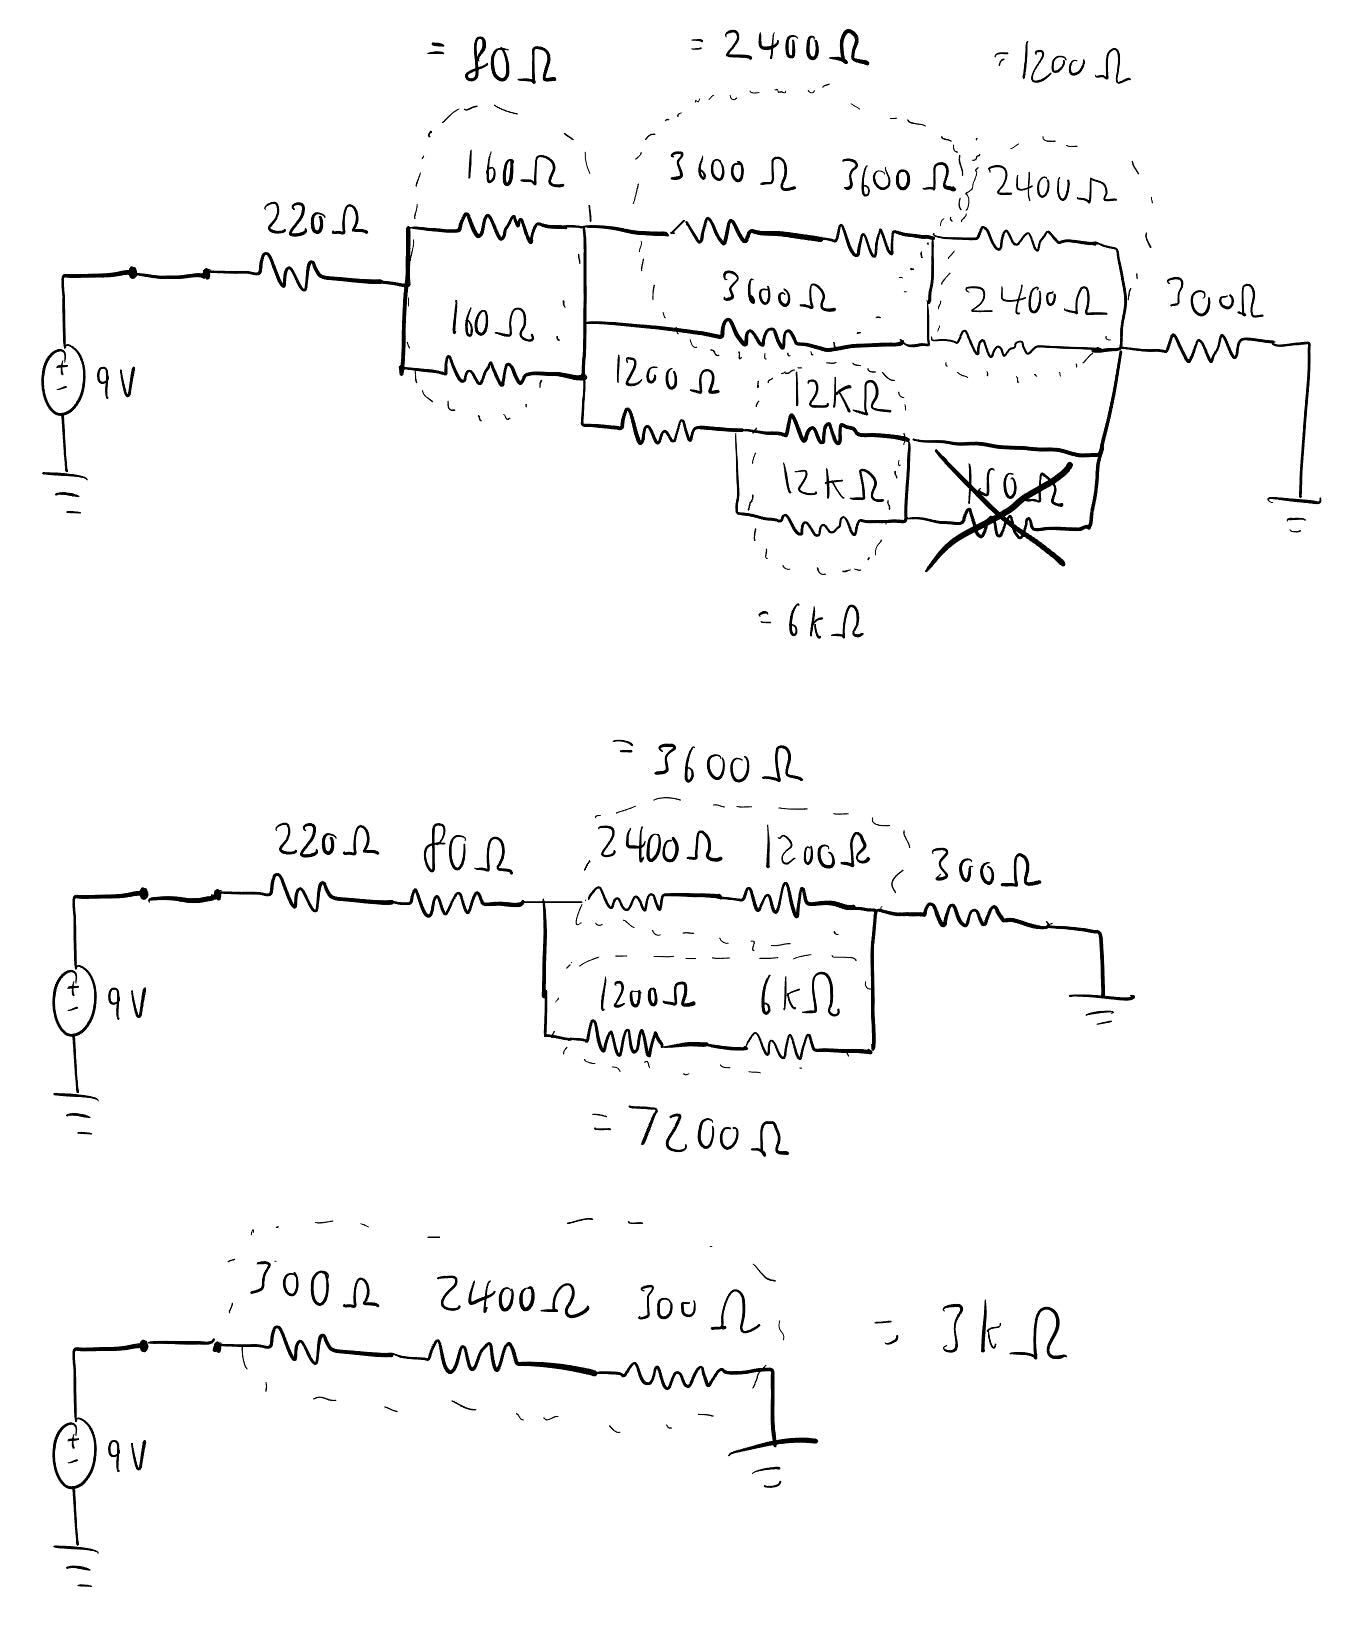
\includegraphics[width=1\textwidth]{image.jpg}
\end{figure}
The equivalent series resistance is 3000$\Omega$. This means the current flowing through
the battery is 9V/3000$\Omega$ = 3mA.

\end{document}